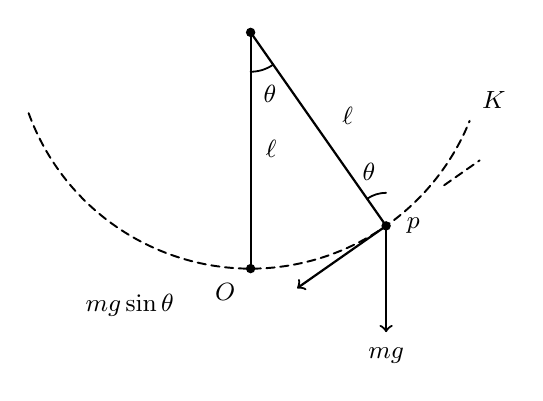
\begin{tikzpicture}[
  x=1cm,
  y=1cm,
  line cap=round,
  line join=round,
  every node/.style={font=\small}
]
  % 以悬点为圆心，O 和 p 同在半径为 l 的圆弧上。
  \def\radius{3}
  \def\swingangle{35}
  \pgfmathsetmacro{\px}{\radius*sin(\swingangle)}
  \pgfmathsetmacro{\py}{\radius-\radius*cos(\swingangle)}
  \pgfmathsetmacro{\topEndAngle}{270+\swingangle}
  \pgfmathsetmacro{\pEndAngle}{90+\swingangle}
  \pgfmathsetmacro{\pLabelAngle}{90+\swingangle/2}

  \coordinate (C) at (0,\radius);
  \coordinate (O) at (0,0);
  \coordinate (P) at (\px,\py);
  \coordinate (Kleft) at ({\radius*cos(200)},{\radius+\radius*sin(200)});
  \coordinate (Kright) at ({\radius*cos(338)},{\radius+\radius*sin(338)});
  \coordinate (TopAngleStart) at ({0.50*cos(270)},{\radius+0.50*sin(270)});
  \coordinate (TopAngleLabel) at ({0.82*cos(270+\swingangle/2)},{\radius+0.82*sin(270+\swingangle/2)});
  \coordinate (PAngleStart) at ({\px+0.42*cos(90)},{\py+0.42*sin(90)});
  \coordinate (PAngleLabel) at ({\px+0.72*cos(\pLabelAngle)},{\py+0.72*sin(\pLabelAngle)});

  % 轨道圆弧，以原图的悬点为圆心。
  \draw[densely dashed, line width=0.7pt]
    (Kleft) arc[start angle=200,end angle=338,radius=\radius cm];

  % 悬点到最低点和质点的两条半径。
  \draw[line width=0.8pt] (C)--(O);
  \draw[line width=0.8pt] (C)--(P)
    node[pos=0.56,above right=2pt] {$\ell$};
  \node[right=2pt] at (0,1.52) {$\ell$};

  % p 点处的切线及重力、切向分量。
  \pgfmathsetmacro{\tangentStartX}{\px+0.90*cos(\swingangle)}
  \pgfmathsetmacro{\tangentStartY}{\py+0.90*sin(\swingangle)}
  \pgfmathsetmacro{\tangentEndX}{\px+1.45*cos(\swingangle)}
  \pgfmathsetmacro{\tangentEndY}{\py+1.45*sin(\swingangle)}
  \pgfmathsetmacro{\componentEndX}{\px-1.38*cos(\swingangle)}
  \pgfmathsetmacro{\componentEndY}{\py-1.38*sin(\swingangle)}
  \draw[densely dashed, line width=0.7pt]
    (\tangentStartX,\tangentStartY)--(\tangentEndX,\tangentEndY);
  \draw[->,line width=0.8pt] (P)--(\px,\py-1.35)
    node[below=2pt] {$mg$};
  \draw[->,line width=0.8pt] (P)--(\componentEndX,\componentEndY);
  \node[anchor=east] at (-0.85,-0.46) {$mg\sin\theta$};

  % 两处角标相同：摆杆与竖直方向的夹角。
  \draw[line width=0.65pt] (TopAngleStart)
    arc[start angle=270,end angle=\topEndAngle,radius=0.50cm];
  \node at (TopAngleLabel) {$\theta$};
  \draw[line width=0.65pt] (PAngleStart)
    arc[start angle=90,end angle=\pEndAngle,radius=0.42cm];
  \node at (PAngleLabel) {$\theta$};

  \fill (C) circle (1.7pt);
  \fill (O) circle (1.7pt);
  \fill (P) circle (1.7pt);
  \node[below left=2pt] at (O) {$O$};
  \node[right=4pt] at (P) {$p$};
  \node[above right=1pt] at (Kright) {$K$};
\end{tikzpicture}
